\documentclass[../nirs.tex]{subfiles}

\begin{document}
\section{Теоретическое изучение предметной области. Построение теоретических
математических моделей}

Система ТО значительно влияет на реализуемые показатели качества автомобильной
техники и эффективность самой ее эксплуатации. Она определяет стратегию
обеспечения работоспособности автомобильного парка, создавая нормативную базу,
которая обеспечивает принятие рациональных решений и условия для контроля
качества технологических процессов.

Система ТО занимает важное место в концепции управления качеством автомобилей.
Сфера эксплуатации влияет на следующие реализуемые показатели качества:

\begin{itemize}

    \item интенсивность изменения показателя качества;

    \item срок службы;

    \item начальные показатели качества.

\end{itemize}

По данным исследований удовлетворительное выполнение рекомендаций системы ТО
обеспечивает в среднем повышение коэффициента технической готовности на 2,5 --
3\%, наработок на отказы и неисправности по различным узлам и механизмам в 1,2
-- 1,9 раз, сокращение расхода топлива на 1,5 -- 3,0\%.

Применяемые системы технического обслуживания автотранспортной техники
базируются на определенных стратегиях обеспечения работоспособности. Всю
возможную совокупность наиболее типичных отказов и неисправностей автомобиля
можно подразделить на две большие группы: профилактируемые и
непрофилактируемые. К последним относятся, во-первых, отказы и неисправности,
которые невозможно заранее предвидеть у конкретного автомобиля, т.е. внезапные;
во-вторых, отказы и неисправности, которые нецелесообразно предотвращать по
экономическим или иным критериям. Таких отказов и неисправностей у современных
автомобилей около 27-39\% от общего числа. Для них действует стратегия \rom{2}
(рисунок \ref{fig:pdf.a}), смысл которой заключающаяся в том, что они
устраняются по мере возникновения. Иногда ее называют \textquote{стратегией
ожидания ремонта}. Если в качестве целевой функции принять затраты, то для
стратегии \rom{2} удельные затраты на ремонт:

\begin{equation*}
    C^{\rom{2}} =
    c\,/\,\bar{x} =
    c : \int_{x_{min}}^{x_{max}} x f(x)\,dx,
\end{equation*}
где $\bar{x},\,x_{min} \,\text{и} \,x_{max}$ -- соответственно средняя,
минимальная и максимальная наработки на отказ; $c$ -- разовые затраты на
устранение отказа; $f(x)$ -- плотность вероятности наработки на отказ.

\begin{figure}[H]
\centering
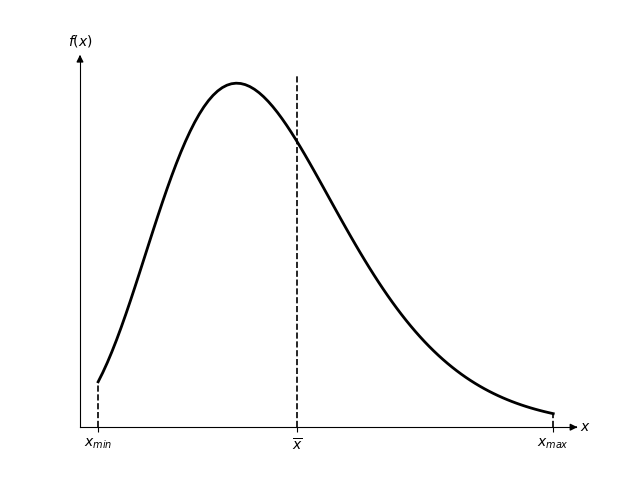
\includegraphics[keepaspectratio,width=\textwidth]{./images/pdf.a.png}
\caption{Стратегия обеспечения работоспособности с использованием стратегии
устранения отказов по потребности}
\label{fig:pdf.a}
\end{figure}

Преимуществом данной стратегии является простота ее реализации. Основным
недостатком -- неопределенность состояния конкретного изделия, которое может
отказать в любое время, а также трудность планирования и организации
технического обслуживания парка.

Для профилактируемой группы отказов и неисправностей может применяться как
стратегия поддержания (проведение технического обслуживания), так и стратегия
восстановления (ремонт) работоспособности. Выделение из этой группы
профилактируемых отказов и неисправностей производится исходя из заданных
критериев эффективности, например обеспечения необходимых уровней безопасности
движения, минимизации затрат ТО, повышения уровня работоспособности,
сокращения расхода топлива и т.д., причем критерии эффективности могут меняться
исходя из конкретных условий и ограничений.

Стратегия \rom{1} -- профилактическая, предусматривает предупреждение
значительной доли отказов и неисправностей данного наименования, восстановление
исходного или близкого к нему технического состояния изделия до того, как
произойдет поломка автомобиля. Поэтому разовые затраты на одно воздействие на
поддержание работоспособности по стратегии \rom{1} ($d_{\text{п}}$), как
правило значительно ниже соответствующих затрат стратегии \rom{2} ($c$), т.е.
$c \gg d_{\text{п}}$, что и является основным источником эффективности
профилактической стратегии. Она реализуется при предупредительном техническом
обслуживании, диагностике, предупредительных заменах деталей. При использовании
стратегии \rom{1} устанавливается наработка (периодичность ТО), по окончанию
которой автомобилю восстанавливают исходное или близкое к нему техническое
состояние (рисунок \ref{fig:pdf.b}).

\begin{figure}[H]
\centering
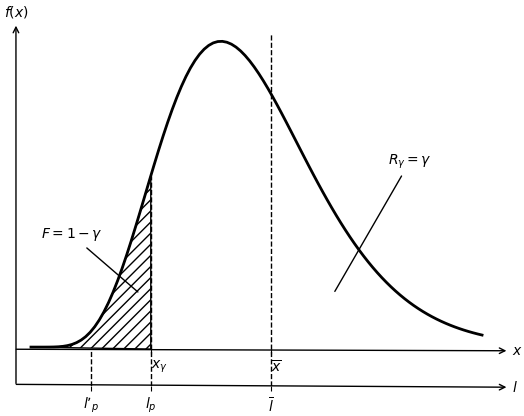
\includegraphics[keepaspectratio,width=\textwidth]{./images/pdf.b.png}
    \caption{Стратегия обеспечения работоспособности с использованием стратегии
    предупреждения отказов (поддержание работоспособности по наработке)}
\label{fig:pdf.b}
\end{figure}

Применяются два основных метода реализации стратегии \rom{1}: планирование
воздействий по наработке с доведением параметра технического состояния до нормы
(\rom{1} -- 1, рисунок \ref{fig:pdf.b}); планирование контроля параметра
технического состояния по наработке с доведением до нормы в зависимости от
фактического и допустимого значений параметра технического состояния (\rom{1} --
2, рисунок \ref{fig:pdf.c}). Поэтому при стратегии \rom{1} профилактическая
операция в общем виде состоит из двух частей -- контрольной и исполнительской:
\begin{equation*}
    d_{\text{п}} = d_{\text{к}} + k d_{\text{и}}\,,
\end{equation*}
где $d_{\text{п}}$ -- стоимость ТО (профилактики); $d_{\text{к}}$ -- стоимость
контрольно-диагностической части операции ТО; $k$ -- коэффициент повторяемости
исполнительской части операции ТО; $d_{\text{и}}$ -- стоимость исполнительской
части операции ТО [\ref{ref:кузнецов}, стр. 170].

\begin{figure}[H]
\centering
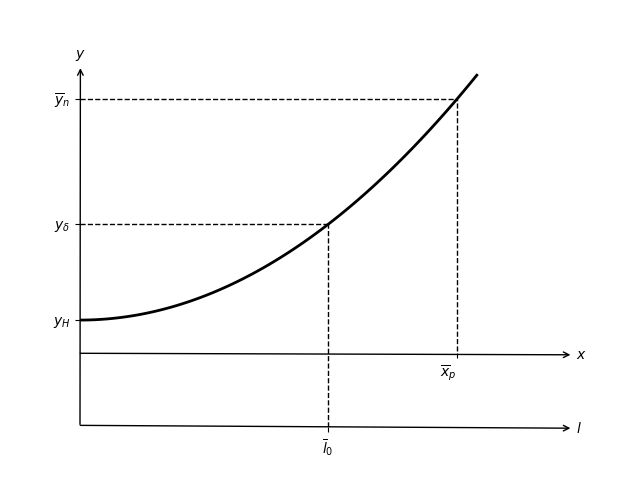
\includegraphics[keepaspectratio,width=\textwidth]{./images/pdf.c.png}
\caption{Стратегия обеспечения работоспособности. Предупреждение отказов
    (поддержание работоспособности по наработке)}
\label{fig:pdf.c}
\end{figure}


\end{document}
